% Chapter Template

\chapter{Arbitrage Theory In Continuous Time Finance} % Main chapter title

\label{Chapter2} % Change X to a consecutive number; for referencing this chapter elsewhere, use \ref{ChapterX}

Arbitrage theory in continuous time finance is a field with a lot of technical details from probability theory and stochastic calculus, where we follow the style in \parencite{Hull} and \parencite{finKont} to focus on intuition without going into the whelm of technicalities and proofs. The focus on this chapter will to provide the basic tools and intuition for the arbitrage theory and lay the foundations for the computational finance methods. The key question is how to price derivative fair and hedge the risk imposed by the derivative. The thesis will mainly deal with the former, where the concepts of arbitrage and replication will be important.\\

We start with introducing the financial markets and key concepts for building arbitrage free and complete market models (see section \ref{FinMarket}). Then we build a framework for finding "fair" prices, i.e. finding a complete model with absense of arbitrage (see section \ref{MultiDimModel}). Lastly we go into specific cases where either a closed-form solution exist or numerical methods is needed (section \ref{classicBS} and \ref{AmericanOptions}).

%----------------------------------------------------------------------------------------
%	SECTION 1
%----------------------------------------------------------------------------------------

\section{Financial Markets}\label{FinMarket}
In the financial markets there is a lot of players and different types of investments. The classical investment types are bonds and stocks, where the big players in the markets are commercial banks, investment banks, insurance companies and pension funds. Besides the classical investments types are derivatives that gives additional options for investment. A derivative or a contingent cliam is a financial instrument depending on an underlying asset, where the dependency is specified in the contract. We will focus on contingent claims with one or two underlying stocks, i.e. univariate and bivariate contingent claims, but the techniques developed can easily be extended to other types of derivatives or multivariate contingent claims. To find prices of contingent claims in modelling we restrict our financial market to d risky assets $\bm{S}(t)=(S_1(t), S_2(t),\ldots, S_d(t))$ and a bank account $S_0(t)$ as numeraire. The probability space $(\Omega, \mathcal{F}, P)$ with a filtration $\mathbb{F}=(\mathcal{F}_t)_{t\geq 0}$ is the fundamental for modelling stochastic processes describing asset prices and trading strategies, where in the thesis the probability space $(\Omega, \mathcal{F}, \mathbb{F}, P)$ will be implicit assumed. Intuitively the filtration $\mathcal{F}_t$ is the information observable to time t, where the filtration $\mathbb{F}^{W}$ is often used in the thesis and it is generated by the wiener processes $(W_t)_{0\leq t \leq T}$. The bank account is assumed to be a strictly positive adapted process $S_0=(S_0 (t))_{t \geq 0}$ and $S_0(0)=1$, where the d risky assets are modelled by a $\mathbb{R}^d$ adapted stochastic proces $\bm{S}=(\bm{S}(t))_{t\geq 0}$. The risky assets are stocks where the stocks are assumed positive $S_i(t)\geq 0$ P-a.s for all i and t by financial reasons. By using the bank account as numeraire i.e. dividing dividing the traded asset by the bank account ($\frac{\bm{S}(t)}{S_0 (t)}$), this amounts to working with \textit{zero interest}. We assume that the our financial market is frictionless.
\theoremstyle{assumption}
\begin{assumption}{\textbf{Frictionless Market: }}\label{EfficientMarket}
We assume following institutional facts:
\begin{enumerate}
\item[•] Short positions and fractional holding are allowed 
\item[•] There are no bid-ask spread, i.e. selling price is equal to buying price
\item[•] There are no transactions costs, taxes or margin requirements of trading.
\item[•] The market is completely liquid, i.e. it is possible to buy/sell unlimited quantities on the market. You can borrow unlimited amount from the bank by short selling.
\end{enumerate}
(see p. 6 \parencite{finKont})
\end{assumption}
Besides the assumptions in \parencite{finKont} will we assume the market gives same uniform price for borrowing money and stocks are fixed stochastic processes exogenously and a priori given. All the assumptions is not realistic in real financial markets, but it gives a reasonable approximation.  The assumptions can be modified but this complicates the mathematical convience, but the financial market is the key to price derivative in arbitrage teory.

%-----------------------------------
%	SUBSECTION 1
%-----------------------------------

\subsection{Contingent Claims}
A contingent claim is a contract on a underlying asset or assets, where the price of the claim is contingent on the price behavior of the underlying asset. We investigate stock derivatibves with different types of contracts, where we will mainly divide the derivatives into two classes. 
\begin{enumerate}
\item Simple stock derivatives (T-claims - european options)
\item Exotic stock derivatives (e.g. American options)
\end{enumerate}
The first class are simple because you can only exercise them at maturity (time T). Actually, we have a closed form solution for european options (section \ref{BS-price-EuroCall}). The exotic derivatives are a broad class of functions on the underlying assets, where you can e.g. have an american option where the holder can exercise from inception to maturity (see section \ref{AmericanOptions}) or a contract on several underlying stocks.

\theoremstyle{definition}
\begin{definition}{\textbf{European Call And Put Option:}}\label{def:CallOptions}
A European call option is an option where the owner of the option has the option to buy the underlying asset to price K at maturity. If the owner of the option chooses to buy the underlying asset, then the option is exercised. The contract function for the european call option:
\begin{equation}
\begin{split}
\Phi(S(T))=\max\{S(T)-K, 0\}
\end{split}
\end{equation}
The put option is the right to sell the underlying asset to price K at maturity, hence the contract function for the european put option is:
\begin{equation}
\begin{split}
\Phi(S(T))=\max\{K-S(T), 0\}
\end{split}
\end{equation}
Where S(T) is the price of underlying asset at maturity and K is the agreed strike price.
\end{definition}

The american option adds the feature to the option, that you can exercise at anytime beetween inception of the contract until maturity. This feature makes the american option an optimal stopping problem and the exercise gain for the american options is called the intrinsic value (section \ref{AmericanOptions}). For the american put option the payoff function at the stopping time is the same as for the european put at maturity. 

\begin{figure}[H]
\centering
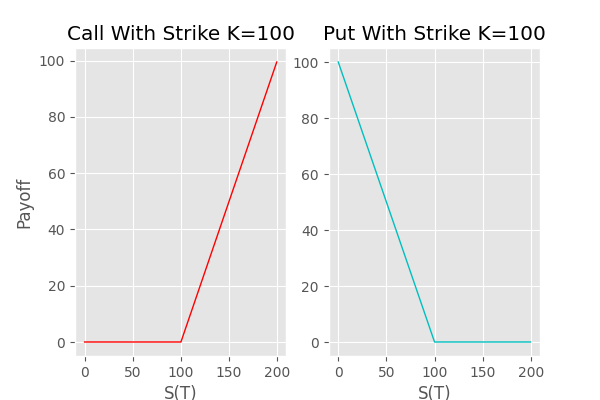
\includegraphics{Figures/contractfct.png}\\
\decoRule
\caption[Contract Functions]{European options payoff at maturity with strike K=100}
\label{fig:contractfct}
\end{figure}

From the above illustration is it clear, that the owner of the option has limited downside, but the illustation does not take into account the initial price for the option. The profit and loss ($P\& L$) graph is also a common way of illustrating the payoff for an option, where you take the initial cost of buying the option into account. The fair price for such type of contract and other contracts will be the topic for this thesis, where the concepts of completeness and arbitrage will be central.

%-----------------------------------
%	SUBSECTION 2
%-----------------------------------

\subsection{Self-financing Portfolio (Without Consumption)}
Before being able to use the concepts of arbitrage and compleness, the construction of the portfolio from the financial market model will be important. The portfolio is the number of each assets of the market the owner of the portfolio holds. The value of the portfolio for a market model with the bank account and d stocks:
\begin{equation}
V^h(t)=\sum_{i=0}^{d} h_{i}(t) S_i(t)
\end{equation}
$V^h$ is called the value process and $h_i(t)$ is number of shares of type i during the period "$[t,t+dt)$". For the definition of arbitrage (Definition \ref{Arbitrage}) we need to restrict ourselfes to self-financing (S-F) portfolios. A self-financing portfolio h, is a portfolio h which doesn't get any external injection of money.
\theoremstyle{definition}
\begin{definition}{Self-financing portfolio}
A portfolio consisting of d+1 assets: \\
h(t)=($h_0(t),h_1(t), \dotsc, h_{d}$) is self-financing if:
\begin{equation}\label{SF}
\begin{split}
dV^{h}(t)=\sum_{i=0}^{d} h_{i}(t) dS_{i}(t)
\end{split}
\end{equation}
Where $S_{i}$ is the $i'th$ asset in our portfolio, d+1 is the total number of assets in our market model and\\
$V^{h}(t)=\sum_{i=0}^{n} h_{i}(t) S_{i}(t)$\\
\end{definition}
When dealing with discrete time finance the S-F portfolio is actually a budget restriction, this is important intuition for the continuous time version, because the continuous time version can be thought of the limit of the discrete version by letting step sizes in time tending to zero. To avoid pathological effects on the portfolio one often introduce the concept of an admissible portofolio:
\theoremstyle{definition}
\begin{definition}{a-admissible portfolio}
For $a\geq 0$, a portfolio h is called a-admissible if its value process $V^h(t)$ is uniform bounded from below by -a. A portfolio h is admissible if it is a-admissible for some $a\geq 0$.
\end{definition}
The definition of a-admissible portfolio to avoid situations as the doubling strategy known from gambling and imposes a limit to the debt arrangement. The important takeaway is that the S-F portfolio is a portfolio where you only reallocate your assets through time within the portfolio.

%-----------------------------------
%	SUBSECTION 3
%-----------------------------------
\subsection{Arbitrage}
Arbitrage is the financial term for a "free lunch". An arbitage opportunity produces something out of nothing without risk, where the efficient market assumptions tells us in a well function market the "money pumps" cannot exist for long, because they would quickly be corrected by exploitation. In order to avoid making a "money machine" in our market, we want to price derivatives by not introducing arbitrage to the market.  
\theoremstyle{definition}
\begin{definition}{\textbf{Arbitrage}:}
An arbitrage possibility on a financial market is an admissible self-financed portfolio h suct that
\begin{equation}\label{Arbitrage}
\begin{split}
V^{h}(0)=0\\
P(V^{h}(T)\geq 0)=1\\
P(V^{h}(T)>0)>1
\end{split}
\end{equation}
The financial market $\bm{S}$ is called arbitrage-free if there exist no arbitrage opportunities. Sometimes $\bm{S}$ is said to satisfy (\textit{NA})\\
(p. 96 \parencite{finKont})
\end{definition}
From the above definition we see that arbitrage is a natural financial requirement for a financial market model, because the investor in a arbitrage portfolio starts with 0 dollars, and without injecting any money, the investor is certain of not losing any money. In addition he has a positive probability by ending up with more than 0 at maturity this cannot be a well function market for both buyers and sellers. To price the derivatives fair in the model, the derivative should not introduce arbitrage to the market. There are different versions of the (\textit{NA}) definition, where for our purpose the above defition is sufficient. The \textit{NA} is not only desirable for the market, we would also like to be able to replicate the payoff of the derivative with the other assets in the financial market model. If every derivative can be replicated in the market, then we have a complete market. 

%-----------------------------------
%	SUBSECTION 4
%-----------------------------------

\subsection{Complete Market And Replication}
The replication argument in Black-Scholes paper \parencite{B-S-Paper} was groundbreaking in the sense that the attitude to risk was irrelavant for pricing, because by continuous trading in the underlyings of the contingent claims cash flow could be replicated. The replication argument shows that the price is unique under the assumption investors prefer more to less. Replication is also important for risk management of the derivative books, because it tells you have to risk neutralize your exposure. A replication or hedge is simply a risk neutralization action in order to minimize the overall risk. In the definition below, we define a hedge for an simple T-claim.
\theoremstyle{definition}
\begin{definition}{\textbf{Hedging and completeness for T-claim}:}
A T-claim X can be hedged, if there exist a self-financing portfolio h such that:
\begin{enumerate}
\item[•] $V^{h}(T)=X$ P-a.s.
\end{enumerate}
I.e. h is an hedge portfolio for X if it is guaranteed to pay in all circumstances an amount identical to the payout of X.\\
The market is complete, if every derivative is hedgeable.
(p. 192 \parencite{finKont})
\end{definition}

By introducing the basic concepts for how to price fair and protect ourselves against financial risk, we will in next section focus on building the financial market model.

%----------------------------------------------------------------------------------------
%	SECTION 2
%----------------------------------------------------------------------------------------

\section{Multidimensional Models}\label{MultiDimModel}
There is two main method for deriving arbitrage free and complete markets. The classical approach is the delta hedging approach \parencite{B-S-Paper} and \parencite{CRR}). The more advanced mathematical approach is the martingale approach  \parencite{finKont}. In this section will we focus on the martingale approach and show that delta hedging approach coincides with the more general martingale theory. For the martingale approach the First and Second Fundamental Theorems of Mathematical Finance will be the key for obtaining a fair market. Besides the model assumptions will we also assumes the financial market assumptions in section \ref{FinMarket}.

\subsection{Model Assumptions}
Let us consider a filtered probability space $(\Omega, \mathcal{F}, P, (\mathcal{F}_t^{\bar{W}})_{t \in [0,T]})$. Note the assumption that filtration is generated from the Wiener process and we consider a finite horizon. we assume $\bar{W}_i$ is k-dimensional and $\bar{W}$ is the only random source . I.e. we assume that we are in a Wiener world, where all processes are Wiener driven. A priori we assume a market $(B(t),S_1(t), S_2(t),\ldots, S_d(t))$, where ${S_i(t)}_{i=1,2,\ldots,d}$ are d risky assets and B(t) is the risk free asset. By assumptions their dynamics are given by:\\
\begin{align}
d\bm{S}(t)&=D[\bm{S}(t)]\bm{\alpha}(t)dt+D[\bm{S}(t)]\bm{\sigma}(t)d\bar{\bm{W}}(t) \quad & S_i(0) &\in \mathbb{R}^+ \label{GBM-P} \\
dB(t)&=r(t)B(t)dt \quad & B(0) &= 1
\end{align}
We assume $\alpha_i$, $\sigma_{ij}$ and the short rate $r(t)$ are adapted processes, this condition are necassary for the stochastic integrals to be well-defined. The evolution of the stocks are described by a geometric brownian motion (GBM) which has a solution to the SDE. The randomness comes from the brownian motion (BM) in the GBM, which has wildly tracjectories. The function $t\mapsto W_{t}(\omega)$ from $[0,\infty)$ to $\mathbb{R}$ is continuosus, but nowhere differentiable. Furthermore has the BM nonzero quadratic variation and infinite variation, which is the reason to stochastic calculus pioneered by Itô. The BM has also well-behaved property e.g. it is a Lévy process, i.e. $W(0)=0 \ a.s$, independent and stationary increments $W(t)-W(s)$ which is normally distributed with mean zero and variance t-s. The brownian motion in the GBM formalizes "random shocks" $dW$ to the stock return with volatility $\sigma$ and $\alpha$ is the drift. Figure \ref{fig:BM} illustrates three approximations to sample paths of the stocks with GBM assumption with initial value $S_{i}(0)=36$.

\begin{figure}[H]
\centering
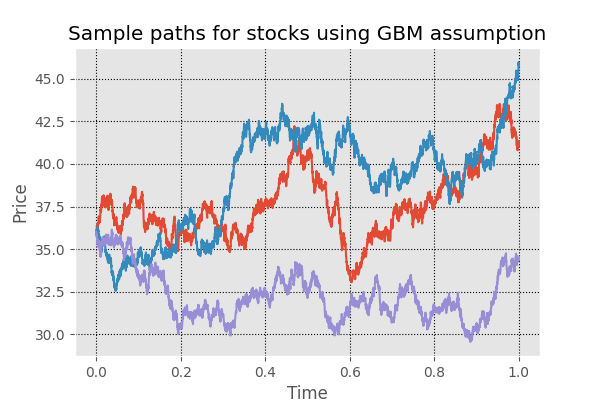
\includegraphics{Figures/samplePath.png}
\decoRule
\caption[Sample Path For Stocks]{Three sample paths for stocks under GBM assumptions, where the spot is \$36, $\sigma$=0.2 and $\alpha$=0.06}
\label{fig:BM}
\end{figure}


The tool for handling BM is stochastic calculus in continuous time, because the standard calculus will not work for the wildly behaved BM. In the representation of the GBM, we used vector and matrix notation for the GBM process. The stock vector is d dimensional and the wiener process vector is k dimensional. The volatility matrix is given by $\bm{\sigma}(t)=\{\sigma_{ij}(t)\}_{i=1,\ldots,d,j=1,\ldots,k}$ and the local mean of rate of return vector is $\alpha(t)=(\alpha_1(t), \alpha_2(t), \ldots, \alpha_d(t))^T$. D(x) denotes a diagonal matrix with vector x as its diagonal and the Wiener processes instantaneous correletion matrix $\rho$ is $Cov(dW_i(t)dW_j(t))=\rho_{ij}dt$.

\subsection{Arbitrage Free Model}
The first problem we are faced with in arbitrage theory is to create a model with no arbitrage opportunities. The First Fundamental Theorem tells us how to not introduce arbitrage to our market model.
\begin{theorem}\label{FFT1}
\textbf{First Fundamental Pricing Theorem of Mathematical Finance(FFT1): } The market model is free of arbitrage if and only if there exist a equivalent martingale measure, i.e. a measure $Q\sim P$ s.t. the processes:
$$\frac{S_0(t)}{S_0(t)}, \frac{S_1(t)}{S_0(t)}, \cdots, \frac{S_d(t)}{S_0(t)}$$
are (local)martingales under Q.
(see p. 154 \parencite{finKont})
\end{theorem}
The processes are martingales is natural, because a martingale is mathmatical formulation that the expected value of the discounted value coincides with the known spot value. In gambling a martingale resembles a "fair" game, which is the same idea for FFT1. By choosing the bank account $B(t)$ as numeraire it follows from the FFT1.

\theoremstyle{proposition}
\begin{proposition}{}
We assume that $B(t)=S_0(t)$ is our numeraire and all the processes are Weiner driven, then a equivalent measure $Q \sim P$ is martingale measure if and only if all assets $(B(t), S_1(t), \ldots, S_d(t))$ have the short rate as their local rates of return, i.e.
\begin{align}
dS_i(t)=S_i(t)r(t)dt+S_i(t)\sigma_i(t)dW^Q(t)
\end{align}
(see p. 154 \parencite{finKont})
\end{proposition}
So to not introduce arbitrage to the model for the financial market, we need to ensure the Q-dynamics of S is:
\begin{equation}\label{Q-dym}
dS(t)=D[S(t)]r(t)dt+D[S(t)]\sigma(t)d{W}(t)
\end{equation}
The tool to obtain the dynamics in eq. (\ref{Q-dym}) is Girsanov theorem (see \ref{Girsanov}). Girsanov theorem is a continuous measure transformation, where in our model we want to transform the dynamics given with the objective probability measure P to an equivalent martingale measure Q (i.e. the martingale measure chosen by the market). By suitable chooses of the likelihood process L and setting $dQ=L(T)dP$, then with Girsanov theorem the transformed process is still a brownian motion:
$$d\bar{W}(t)=\phi(t)dt + dW(t)$$
When applying to eq. (\ref{GBM-P}):
$$dS(t)=D[S(t)](\alpha(t)+\sigma(t)\phi(t))dt+D[S(t)]\sigma(t)d{W}(t)$$
Going back to the FFT1 and the proposition, we know that Q is martingale measure if and only if:
\begin{align}\label{marketPriceOfRisk}
\bm{\alpha}(t)+\bm{\sigma}(t)\bm{\phi}(t)=\textbf{r}(t) \quad holds \ with \ probability \ 1 \ for \ each \ t
\end{align}
We disregard pathological models when doing so the term generically arbitrage free will be used. 

\theoremstyle{definition}
\begin{definition}{\textbf{Generically arbitrage free}:}
The model in this section is said to be generically arbitrage free if it is arbitrage free for every (sufficiently integrable) choice of $\bm{\alpha}$.
(p. 198 \parencite{finKont})
\end{definition}

Furthermore we assume enough integrability and we have the following useful result:
\theoremstyle{proposition}
\begin{proposition}{}\label{arbitrageFreeProp}
Disregarding integrability problems the model is generically arbitrage free if and only if, for each $t\leq T$ and P-a.s. the mapping:
$\bm{\sigma}(t):\mathbb{R}^k \to \mathbb{R}^n$ is surjective, i.e. if and only if the volatility matrix $\bm{\sigma}(t)$ has rank n.
(see p. 198 \parencite{finKont})
\end{proposition}
We note that in order not to have arbitrage in our model, we need $k\geq n$, i.e. have at least as many random sources as number of risky assets.

\subsection{Complete model}
Second Fundamental Pricing Theorem is key to obtain a complete market model, i.e. a market model where every claim can be hedged.
\begin{theorem}\label{FFT2}
\textbf{Second Fundamental Pricing Theorem of Mathematical Finance(FFT2): } Assuming absence of arbitrage, the market model is complete if and only if the martingale measure $Q$ is unique.
(see p. 155 \parencite{finKont})
\end{theorem}
In our Wiener world we have a unique martingale measure if eq. \ref{marketPriceOfRisk} has a unique solution, where from the proof of the proposition \ref{completeProp} is clear why the Wiener world assumption is required. If we had more random sources e.g. a poisson process, than there is no guarentee that the equivalent measure transformation is of the Girsanov type above. 

\begin{proposition}{}\label{completeProp}
Assume that the model is generically arbitrage free and that the filtration is defined by:
$$\mathcal{F}_t=\mathcal{F}_t^{\bar{W}} \quad t \in [0,T]$$
Then disregarding integrability problems, the model is complete if and only if k=n and the volatility matrix $\sigma(t)$ is invertible P-a.s. for each $t \leq T$
\begin{proof}
The proof is based on martingale representation theorem \ref{MRT} (MRT) and converse of Girsanov theorem \ref{ConverseGirsanov} which uses MRT, hence the assumption about the only randomness comes from the wiener process. By the two theorems we know every equivalent meassure transformation is obtained by Girsanov theorem of the above type. Hence the martingale measure is unique if anf only if the solution to \eqref{marketPriceOfRisk} is unique (p. 200 \parencite{finKont}).                                         
\end{proof}
\end{proposition}
Intuitively we need one independent traded assets excluding the bank account for every source of randomness (Meta-theorem 8.3.1 \parencite{finKont}).


\subsection{Pricing and connection to classical approach}
The pricing formula for arbitrage free market model is the risk neutral valuation formula:
\begin{proposition}{\textbf{Risk Neutral Valuation Formula}}\label{RNVF}
To avoid arbitrage, $\mathcal{X}$ must be priced according to the formula:
\begin{align}
\Pi(t;\mathcal{X})=S_0(t)E^Q[\frac{\mathcal{X}}{S_0(T)}|\mathcal{F}_t]
\end{align}
Note if we choose our numeraire $S_0(t)=B(t)$ then
\begin{align}
\Pi(t;\mathcal{X})=E^Q[\exp(-\int_t^T r(s) ds) \mathcal{X}|\mathcal{F}_t]
\end{align}
(see p. 155 \parencite{finKont})
\end{proposition}
Proposition \ref{RNVF} will raise the question if there is more than one fair price for the derivative. The answer is found in FTT2, the market is complete if and only if the measure Q is unique. Intuitively it means that if you can replicate the derivative with a S-F portfolio, then the risk free position should only earn risk free interest rate. \\

The classical approach in \parencite{B-S-Paper} to arbitrage free and complete market models is based on a Markovian model assumption. For the model to have markovian property, we assume k=n and the probability space is $(\Omega, \mathcal{F}, P, \mathcal{F}_t^{\bar{W}_t})$. Furthermore we assume $\bm{\alpha}$ and $\bm{\sigma}$ are deterministic and constant over time. $\bm{\sigma}$ is also assumed invertible. Under these more restrictive assumptions the risk neutral valuation formula for a simple T-claim is given by the pricing function:
\begin{align}\label{MarkovRNVF}
F(t,S(t))=\exp(-r(T-t))E^Q[\mathcal{X}|S(t)]
\end{align}
The Markov property implies that the price only depend on the current state of $\bm{S}$, and then applying Kolmogorov backward equation on eg. \ref{MarkovRNVF}, we obtain the BS-PDE for the pricing function F(t,S(t))=$\Pi(t; \mathcal{X})$.

\begin{theorem}\label{BSPDEMultiDim}
\textbf{Black Scholes PDE: } Consider the contract $\mathcal{X}=\Phi(\bm{S}(T))$. In order not to introduce arbitrage to the market, the pricing function $F(t,s)$ must solve the boundary value problem.
\begin{equation}
\begin{split}
F_t(t,s)+\sum_{i=1}^{n} rs_iF_i(t,s)+\frac{1}{2} tr\{\sigma^* D[S] F_{ss} D[S] \sigma\} -rF(t,s)&=0\\
F(T,s)&=\Phi(s)
\end{split}
\end{equation}
(see p. 203 \parencite{finKont})
\end{theorem}


%----------------------------------------------------------------------------------------
%	SECTION 3
%----------------------------------------------------------------------------------------
\section{Classical Black-Scholes Formulas}\label{classicBS}
We will not do the classical delta hedging approach in \parencite{B-S-Paper}. Instead we use the general multidimensional martingale approach to derive the essential formulas for pricing. 
To derive a closed-form solution to the European call and put option, we concentrate at a special case of the multidimensional framework, where we only have the risk free asset and one risky asset in the financial market model. 
We further restrict ourselves to:
\theoremstyle{assumption}
\begin{assumption}{\textbf{Black-Scholes assumptions}:}\label{BS-Assumption}
We assume following ideal conditions in addition to \eqref{EfficientMarket}:
\begin{enumerate}
\item[•] The short-term interest rate r, volatility $\sigma$ and the drift $\alpha$ are constant.
\item[•] The stock pays no dividends or other distributions.
\item[•] The option is a simple option ("European").
\end{enumerate}
(p. 640 \parencite{B-S-Paper})
\end{assumption}

We assume the underlying stock and the bank account have differentials:
\begin{align}
dS(t)&=S(t)\cdot \alpha dt+S(t) \sigma d\bar{W}(t) \quad & S(0) &\in \mathbb{R}^+ \\
dB(t)&=r B(t)dt \quad & B(0) &= 1
\end{align}
By Itô's lemma (lemma \ref{Ito}) for one dimensional process the solution to the differentials above is:
\begin{align}
S(t)&=S(0) \cdot \exp \bigg( (\alpha -\frac{1}{2} \sigma^2) t + \sigma W(t) \bigg) \\
B(t)&=\exp(r\cdot t)
\end{align}
Where $\alpha$ is the local mean rate of return and $\sigma$ is the volatility of S are constants. By above assumptions we are in a Markovian model, and we know that the Black Scholes PDE in this setup (see eq.  \ref{BSPDEMultiDim}) from the risk neutral valuation formula. The solution of the SDE of S under Q dynamics is:
\begin{equation}\label{GBM}
\begin{split}
S(t)=S(0) \cdot \exp \bigg( (r -\frac{1}{2} \sigma^2) t + \sigma W(t) \bigg)
\end{split}
\end{equation}
By eq. \eqref{GBM} we see that the Black-Scholes model assumes that the stock price change continuously in a way that produces a lognormal distribution for the price at any future time. \\

By the simple option assumption the Kolmogorov backward equation for the RNVF gives the BS-PDE. The PDE can then be solved analytically and then we arrive at a closed form solution for european call and put options. The european call and put option can also be derived directly with the RNVF. 

\theoremstyle{proposition}
\begin{proposition}{}\label{BS-price-EuroCall}
\textbf{Black-Scholes formula for call option:} The price of a European call option with strike K and maturity T is given by the formula  $\Pi(t)=F(t,S(t)$, where
\begin{align*}
F(t,s)=c(t,s)=s \cdot N(d_1(t,s)) - e^{-r(T-t)}\cdot K \cdot N(d_2(t,s))
\end{align*}
N is the cumulative distribution function of a standard normal distribution $\mathcal{N}(0,1)$ and
\begin{align*}
d_1(t,s)=\frac{1}{\sigma\cdot \sqrt{T-t}} \cdot \bigg( \ln(\frac{s}{K}) + (r+\frac{1}{2} \sigma^2) (T-t) \bigg)\\
d_2(t,s)=d_1(s,t)-\sigma \sqrt{T-t}
\end{align*}
(see p. 105 \parencite{finKont})
\end{proposition}
We provided only the price for the european call option, but the european put price can easily be obtained by applying the put-call-parity for european options.

\theoremstyle{proposition}
\begin{proposition}{}\label{put-call-parity}
\textbf{Put-call parity:} 
Assume the call and put option has same strike price and time to maturity.
\begin{align*}
p(t,s)=K\cdot \exp(-r(T-t))+c(t,s)-s
\end{align*}
(see p. 126 \parencite{finKont})
\end{proposition}

The aim for this thesis is to price american put options, but the european option provide a reference price in a closed form format. The put-call-parity holds only for european options, where for the american option there is a bound on the difference in price:
$$S_0 - K \leq C-P \leq S_0 - K \cdot e^{-rT}$$

The above formula for the European call option is actually the same for an American call option, but is not true for an American put option or for call options with underlying stock paying dividends. The result for the American call option was shown by Merton \parencite{Merton73}, that the intrinsic value is never greater than the worth of the option given by the risk-neutral valuation formula. In section \ref{AmericanOptions} we will show a martingale approach to prove the value of a European and American call coincides when the underlying is a non-dividend paying stock.

%----------------------------------------------------------------------------------------
%	SECTION 4
%----------------------------------------------------------------------------------------

\section{American Options And Optimal Stopping}\label{AmericanOptions}
The American options adds additional complexity to the pricing problem, because compared to the European option the American option can be exercised at any time from inception to maturity. The exercise value at time t is also called the intrinsic value of the option. This section is inspired by \parencite{finKont, Shiryaev06,Elliott99} where \parencite{Shiryaev06} is specialized to optimal stopping problems, where the two other references gives the fundamental mathematics for option and arbitrage theory in general.\\

We still assume a diffusion setting that the underlying stochastic process for the stock behaves under the risk neutral measure as a GBM.
\begin{equation*}
\begin{split}
S_i(t)=S_i(0) \cdot \exp \bigg( \sum_{j=1}^{d}(\sigma_{i,j} W_j(t) -\frac{1}{2} \sigma_{i,j}^2 t) + rt \bigg) \quad  for \ i=1,\ldots,d
\end{split}
\end{equation*}
Where the Wiener processes are independent and its domain in $\mathbb{R}^+$. The exercise feature of the american option raises the problem of rationally to find the optimal stopping time to maximize profit. The value of the option is given by exercising the option at the optimal stopping time, hence it is a optimal stopping problem. We will assume a finite horizon $T\in \mathbb{R}_*^+$ throughout the thesis, because all the derivative will be priced in a finite timeframe. Let the gain function $G:\mathbb{R}\to \mathbb{R}$ be a measurable function satisfying:
\begin{equation}\label{existAmer}
E_{s}[\sup_{0\leq t \leq T}|G(S(t))|] < \infty
\end{equation}
where $S$ is the underlying stochastic process. If the integrability condition is satisfied on a finite interval $[0,T]$ (equation \eqref{existAmer}) then the optimal stopping problem for gain function G and $s \in \mathbb{R}$ is well defined. We assumed that the underlying stochastic S(t) process is time-homogeneous, but the assumption can be relaxed. If S(t) is a time-inhomegenous we can extend the underlying process S(t) by time albeit increasing the underlying process dimension. We define the optimal value process in terms of the gain process.

\theoremstyle{definition}
\begin{definition}{}\label{optValFunc}
For fixed $(t,x)\in [0,T] \times \mathbb{R}$, and each stopping time $\tau$ with $\tau\geq t$ the optimal value function $V(t,x)$ is defined by
\begin{align}
V(t,x)= \sup_{\tau \in \mathcal{T}^T} E_{t,x}[G(S(\tau))]
\end{align}
A stopping time which realizes supremum for V is called optimal and be denoted $\hat{\tau}$.
(see page 341 \parencite{finKont})
\end{definition}

The solution to the optimal stopping problem $\hat{\tau}$ is where supremum is attained and the price is then $V(t,x)$ for $(t,x)\in [0,T] \times \mathbb{R}$. The supremum is taken over all stopping times with respect to the natural filtration $\mathcal{F}_{t}$ belonging in the class of stopping times:
$$\mathcal{T}_0^T=\{\tau : 0 \leq \tau \leq T \}$$
The definition of a stopping time $\tau$ can be seen in definition \ref{StoppingTime}, where the intuition is that the stopping time is a random time, such that we know at time t wheater to stop. To solve the optimal stopping problem some trivial solutions are immediate by martingale properties:
\begin{proposition}\label{TrivialMG}
The following hold:
\begin{enumerate}
\item[•] If $G(S(t))$ is a submartingale, then it is not optimal to stop at all and $\tau^*=T$
\item[•] If $G(S(t))$ is a martingale, then all stopping times $\tau\in [0,T]$ are optimal
\item[•] If $G(S(t))$ is a supermartingale, then it is optimal to stop immediately. i.e. $\tau^*=0$
\end{enumerate}
(p. 330 \parencite{finKont})
\end{proposition}

Examples of gain functions could be the american call and put options:
\begin{align}
C(t,x)=\sup_{\tau \in \mathcal{T}_t^T} E^Q[\exp(-r(\tau-t)) (S(\tau)-K)^+|S(t)=x] \quad for \ t\in [0,T] \ and \ x\in\mathbb{R}^+\\
P(t,x)=\sup_{\tau \in \mathcal{T}_t^T} E^Q[\exp(-r(\tau-t)) (K-S(\tau))^+|S(t)=x] \quad for \ t\in [0,T] \ and \ x\in\mathbb{R}^+
\end{align}


\subsection{American Call Without Dividends}
The American call options is a special case, because the optimal stopping time is always at the options maturity. With martingale machinery it means the value-process is a submartingale which implies that $\hat{\tau}=T$ (proposition \ref{TrivialMG}). Remember the optimal stopping problem for an american call option:
$$C(t,x)=\sup_{\tau \in \mathcal{T}_0^{T-t}} E_{t,x}^Q[\exp(-r\tau) (S(t+\tau)-K)^+]$$
Looking at the gain function:
\begin{equation*}
\exp(-r\tau) (S(t+\tau)-K)^+ = (\exp(-r t) S_{t} - \exp(-r t) K)^+
\end{equation*}
Recall that the discounted price process $\exp(-r\cdot t) \cdot S_t$ is a Q-martingale and $\exp(-r\cdot t) \cdot K$ is a deterministic decreasing function in t. Furthermore the function $x \mapsto (x)^+$ is convex, hence the gain function is a $Q$-submartingale. The last result used is that a convex and increasing function on a submartingale is still a submartingale, hence the optimal stopping time is $\hat{\tau}=T$.

\subsection{American Put}\label{americanPut}
The arbitrage-free price for an american put at time t:
\begin{equation}\label{AmericanPutPrice}
P(x,t)=\sup_{\tau \in \mathcal{T}_t^T} E^Q[\exp(-r(\tau-t)) (K-S(\tau))^+|S(t)=x] \quad for \ t\in [0,T] \ and \ x\in\mathbb{R}^+
\end{equation}
For the american put we need computational methods, because the american and european value does not coincides like for the call option.

\begin{proposition}{}
Consider european and american out options with same maturity T and strike K. If the risk free rate $r\in \mathbb{R}_*^+$, then for any $t<T$
\begin{equation}
\begin{split}
p(x,t)<P(x,t)
\end{split}
\end{equation}
\begin{proof}
WLOG we assume that t=0. Define the stopping time
$$\tau = min \{t\geq 0 : S(t) \leq K(1-\exp(-r\cdot (T-t)))\}$$
We consider a exercise strategy $min\{\tau, T\}$, where the strategy is not necassary optimal. We consider two events:
\begin{enumerate}
\item[1)] $\tau<T$
\item[2)] $\tau \geq T$
\end{enumerate}
The first case is to exercise at time $\tau$ when $S(\tau) \leq K(1-\exp(-r\cdot (T-t)))$. Here the payoff by exercing will be at least $K\exp(-r\cdot (T-\tau))$. The cashflow receive is then invested into the bank account at time $\tau$. At maturity the strategy gives the holder of the put a payoff K, where the european contract with strike K will pay less, because the stock price at maturity will be $S(T)>0 \ a.s.$
The second case is trivial, because the european and american put will give the same payoff. \\
Since the first case has positive probability, the american put has higher discounted expected payoff by following above strategy regardless of the spot price for the stock. 
\end{proof}
\end{proposition}
The above proposition shows the optimal stopping strategy is not always to hold the option to maturity, hence the theory of optimal stopping is important for pricing of american put options. The american put has consequently no closed form solution, but we can search for a lower exercise boundary b(t) such that the holder of the option should exercise when:
$$S(\tau)\leq b(\tau) \quad \tau \leq T$$
The continuation $C$ and stopping set $\bar{D}$ are given for an american put.
\begin{align}
C=\{(t,x) \in [0,T) \times (0,\infty) : V(t,x) > G(x) \}\\
\bar{D}=\{(t,x) \in [0,T) \times (0,\infty) : V(t,x) = G(x) \}
\end{align} 

Hence the first optimal stopping time after time t for the american put is
\begin{equation}
\begin{split}
\hat{\tau}= \inf\{u \in [t,T] : P(S(u),u) = (K-S(u))^+ \}
\end{split}
\end{equation}



\subsection{Discrete time valuation}\label{DiscreteValueFramework}
To solve the optimal stopping problem numerical methods are required for the american put option, hence the first step is to discretize time. In chapter \ref{Chapter3} will we show two approaches to price an american put option, where both are based on the calculating the conditional expectation of the continuation value. Suppose the probability space $(\Omega, \mathcal{F}, P)$ is equipped with the natural discrete filtration $(\mathcal{F}_{t_n})_{n=0,1,\ldots,N}$ modeling a financial market. By discretization of time we are actually looking at a bermuda option, but for sufficient small time steps the bermuda option approximate the american option well. The tenor structure is that the time to maturity is divided into a grid of N+1 equidistant points in time $0=t_0\leq t_1\leq t_2, \cdots \leq t_N=T$, where $\Delta t_n = t_n-t_{n-1}=T/N$ for each $n=1, \ldots, N$. A bermuda option incepted at time $t_0$ has $\mathcal{T}(t_1,t_2,\ldots,t_N)$ exercise dates or decision points, where the option holder chooses to exercise or keep the option alive. The underlying process is assumed to be markovian with state variables $(S(t_n))_{n=0,1,\ldots,N}$ recording all necessary information about relevant financial variables adapted to the natural filtration in order to solve the optimal stopping problem with the dynamic programming principle. Futhermore is the gain process adapted to the filtration and square integrable $E[\max_{0\leq n \leq N} |G(S(t_n))|^2]<\infty$, which is necassary to use regression on a finite set of functions to approximate the conditional expectation (section \ref{LSM}).\\

The optimal stopping problem in discrete time is to find
\begin{equation}\label{Bermudanstop1}
\sup_{\tau \in \mathcal{T}(0,\ldots,T)} E^Q[G(S(\tau))]
\end{equation}
For using the programmable dynamic programming principle the Snell envelope $(U(t_{n}))_{n=0,1,\ldots, N}$ (definition \ref{snellEnvelope}) of the gain function $G(S(t_n))_{n=0,\ldots,N}$ is useful and defined by
$$U(t_n)=\esssup_{\tau \in \mathcal{T}(n,\ldots, N)} E^Q[G(S(\tau_{t_n}))|\mathcal{F}_{t_n}] \quad n=0,1, \ldots, N$$
The snell envelope $U(t_n)$ is the smallest supermartingale of the gain process $\{G(S(t_n))\}$, i.e. the smallest supermartingale dominating the gain process. Using the Snell envelope theory the optimal stopping problem can be solved with the dynamic programming principle.
\begin{equation}\label{valueIteration}
\begin{split}
\begin{cases}
          U(T) = G(S(t_N))\\
          U(t_n) = max\{ G(S(t_n)), E^Q[U(t_{n+1})|\mathcal{F}_{t_n}])\} \quad for \ n={0,\ldots,N-1} \\ 
\end{cases}
\end{split}
\end{equation}
The equation \eqref{valueIteration} known as value iteration indicates that the holder should exercise the first time $G(S(t_n))> E^Q[U(t_{n+1})|\mathcal{F}_{t_n}])$ in order to maximize payoff from the option, hence we get the first optimal stopping time. Note that an optimal stopping time will always exist in discrete time when $T<\infty$. There is though no guarantee that the stopping time is unique. The value itereation gives the optimal value process of the gain process $G(S(t))$ (theorem \ref{SnellEnvelopeTheorem}). So 
$$U(t_n)=E^Q[G(S(\tau_{t_n})|\mathcal{F}_{t_n}]$$ with 
$$\tau_{t_n}=\min \{ k \geq n : U(t_k)=G(S(t_k)) \}$$ and 
$$E^Q[U(0)]= \sup_{\tau \in \mathcal{T}(0,\ldots, T)} E^Q[G(S(\tau))]=E^Q[G(S(\hat{\tau}))]$$ 
The optimal stopping problem can also be solved in terms of stopping times instead of the using the value process. This alternative dynamic programming principle equation is called policy iteration.
\begin{equation}\label{policyIteration}
\begin{split}
\begin{cases}
          \tau_{t_N} = t_N\\
          \tau_{t_n} = t_n \cdot 1_{\{G(S(t_n)) \geq E^Q[G(\tau_{t_{n+1}})|\mathcal{F}_{t_n}])\}} + \tau_{t_{n+1}} \cdot 1_{\{G(S(t_n)) < E^Q[G(\tau_{t_{n+1}})|\mathcal{F}_{t_n}])\}} \quad for \ n={0,\ldots,N-1} \\ 
\end{cases}
\end{split}
\end{equation}

The first approach, the binomial model, uses the idea of dynamic programming, where the orginal problem is solved iterative by recursive subproblems. The underlying stochastic process is approximated by a discrete binomial recombining lattice, where the iterative scheme makes it easy to calculate both european and american option prices. The american put option can be solved recursively with dynamic programming principle with value iteration: 
\begin{equation}\label{BellmanEq}
\begin{split}
\begin{cases}
          P(t_i) = max\{ (K-S(t_i))^+, \exp(-r\cdot \Delta t) E^Q[P(t_{i+1})|\mathcal{F}_{t_i}])\} \quad for \ i={0,\ldots,N-1} \\
          P(t_N) = (K-S(t_N))^+ 
\end{cases}
\end{split}
\end{equation}

The second approach, Least Square Monte Carlo Method (LSM) model, is to combine dynamic programming and monte carlo simulation, but this method uses the policy iteration principle instead of the value iteration. The method uses regression to calculate the expected continuation value of simulated paths instead of discretization of the underlying stochastic process. By using regression the method overcome the challenge with pure simulation method. In order to find a optimal exercise strategy a series of conditional expectations need to be calculated which are computational expensive to calculate using pure simulation methods. Both methods will be explained in details in chapter \ref{Chapter3}.





